%!TEX TS-program = xelatex
%!TEX encoding = UTF-8 Unicode
\documentclass[reqno ,11pt]{amsart}
\usepackage[foot]{amsaddr}
\usepackage{graphicx}
\usepackage[usenames,dvipsnames]{xcolor}
\usepackage[paperwidth=7in,paperheight=10in,text={5in,8in},left=1in,top=1in,headheight=0.25in,headsep=0.4in,footskip=0.4in]{geometry}
\usepackage{natbib}
\usepackage{subfigure}
\usepackage{lineno}
\usepackage{pdflscape}
\usepackage{afterpage}
\bibpunct[, ]{(}{)}{,}{a}{}{,}
\DeclareMathOperator{\var}{var}
\DeclareMathOperator{\cov}{cov}
\DeclareMathOperator{\E}{E}

\synctex=1

\newcommand*\patchAmsMathEnvironmentForLineno[1]{%
  \expandafter\let\csname old#1\expandafter\endcsname\csname #1\endcsname
  \expandafter\let\csname oldend#1\expandafter\endcsname\csname end#1\endcsname
  \renewenvironment{#1}%
     {\linenomath\csname old#1\endcsname}%
     {\csname oldend#1\endcsname\endlinenomath}}% 
\newcommand*\patchBothAmsMathEnvironmentsForLineno[1]{%
  \patchAmsMathEnvironmentForLineno{#1}%
  \patchAmsMathEnvironmentForLineno{#1*}}%
\AtBeginDocument{%
\patchBothAmsMathEnvironmentsForLineno{equation}%
\patchBothAmsMathEnvironmentsForLineno{align}%
\patchBothAmsMathEnvironmentsForLineno{flalign}%
\patchBothAmsMathEnvironmentsForLineno{alignat}%
\patchBothAmsMathEnvironmentsForLineno{gather}%
\patchBothAmsMathEnvironmentsForLineno{multline}%
}

%\usepackage{lmodern}
%\usepackage{unicode-math}
\usepackage{mathspec}
\usepackage{xltxtra}
\usepackage{xunicode}
\defaultfontfeatures{Mapping=tex-text}
\setmainfont[Scale=1,Ligatures={Common}]{Adobe Caslon Pro}
\setromanfont[Scale=1,Ligatures={Common}]{Adobe Caslon Pro}
\setmathrm[Scale=1]{Adobe Caslon Pro}
\setmathfont(Digits,Latin)[Numbers={Lining,Proportional}]{Adobe Caslon Pro}

\definecolor{linenocolor}{gray}{0.6}
\definecolor{prec}{RGB}{42,115,205}
\definecolor{sens}{RGB}{255,112,0}
\definecolor{spec}{gray}{0.4}
\renewcommand\thelinenumber{\color{linenocolor}\arabic{linenumber}}

\usepackage{fix-cm}

\setcounter{totalnumber}{1}

\newcommand{\mr}{\mathrm}
\newcommand{\prim}{{\;\prime}}

\renewcommand{\baselinestretch}{1.0}

\newcommand{\hatr}[2]{\mkern+#1mu \hat{\mkern-#1mu #2}}

% code for adding space to superscripts in mathmode (helps with Caslon typeface tilt)
\newcommand{\upsup}[1]{\sp{\,#1}}
\begingroup\lccode`~=`^\lowercase{\endgroup\let~\upsup}
\AtBeginDocument{%
  \catcode`^=12
  \mathcode`^="8000
}

\begin{document}

\title[Vocal Repertoires]{\large Estimating Vocal Repertoires From Limited Samples}
\author{Richard McElreath}
\address{Department of Human Behavior, Ecology and Culture, Max Planck Institute for Evolutionary Anthropology, Deutscher Platz 6, 04103 Leipzig, Germany}
\email{richard\_mcelreath@eva.mpg.de}
\date{\today}

\maketitle

{\vspace{-6pt}\footnotesize\begin{center}\today\end{center}\vspace{24pt}}

\linenumbers
\modulolinenumbers[5]

\section{Purpose}

Suppose a population of $N$ individuals (monkeys, people) who produce among them $M$ different vocalizations. Each individual has potentially a different repertoire of these $M$ vocalizations. We want to characterize repertoire at the individual level, so that we might study its relationship with development for example. 

One problem is the undercounting of repertoire which is expected in any finite sample. If some vocalizations are rare, and recordings are short or small in number, then on average we will undercount true repertoire size. 

\section{Modeling strategy}

We seek a vector $\phi$ of posterior probability distributions of length $M$ for each individual $i$. In the case that $i$ was observed to produce a $m$, then $\phi_m$ is 1. But when $m$ was not observed, we can compute the posterior probability that this was due to the finite sample, an undercount. 
In the simplest model, assume that each vocalization $m$ is produced at a rate $\lambda_m$, when an individual possesses it. This produces a Poisson distribution of the counts $Y_{i,j,m}$ of each possessed vocalization $m$ in a focal recording $j$ of duration $d_j$.
\begin{align*}
Y_{i,j,m} &\sim \mathrm{Poisson}(  \lambda_m \, d_j \, x_{i,m} )
\end{align*}
where $x_{i,m}$ is an indicator variable for whether individual $i$ possesses vocalization $m$. 
When the observed $y=Y_{i,j,m}>0$, then the probability is:
\begin{align*}
\Pr(y|y>0) &= p_{m} \frac{( \lambda_m d_j )^y \exp(-\lambda_m d_j) }{ y! }
\end{align*}
where $p_m$ is the probability an individual possesses $m$. When $y=0$ is observed, we require a mixture:
\begin{align*}
\Pr(y|y=0) &= p_{m} \exp(-\lambda_m d_j) + (1-p_{m})(1)
\end{align*}

Let $X_{i,m}$ be the total number of times $i$ was observed to use $m$ and $D_{i}$ be the total sampling effort (duration of recordings). If $X_{i,m}>0$, then $i$ possesses the vocalization. But what about when $X_{i,m}=0$? In that case, the posterior probability that individual $i$ possesses vocalization $m$ follows from Bayes' rule:
\begin{align*}
	\Pr(x_{i,m}=1|X_{i,m}=0,D_{i}) &= \frac{\Pr(0|x_{i,m}=1)\Pr(x_{i,m}=1)}{\Pr(0)} \\ 
	&= \frac{\Pr(0|\lambda_m D_{i})p_m}{\Pr(0|\lambda_m D_{i})p_m + (1-p_m)}
\end{align*}
And this is sufficient to solve the problem.

In the Poisson case, we need only the total duration of the recording. 
This model can be modified to allow for Markov transitions between vocalizations, but then we require time stamps for each vocalization. 

\section*{Implementation}

We developed a generative model of the sampling design, in which each individual has a variable number of recordings of variable length. Then we used Stan to sample from the posterior distribution of the inferred individual repertoires.

First we can ask how well the model recovers the rate $\lambda$ and probability $p$ variables.
\begin{center}
	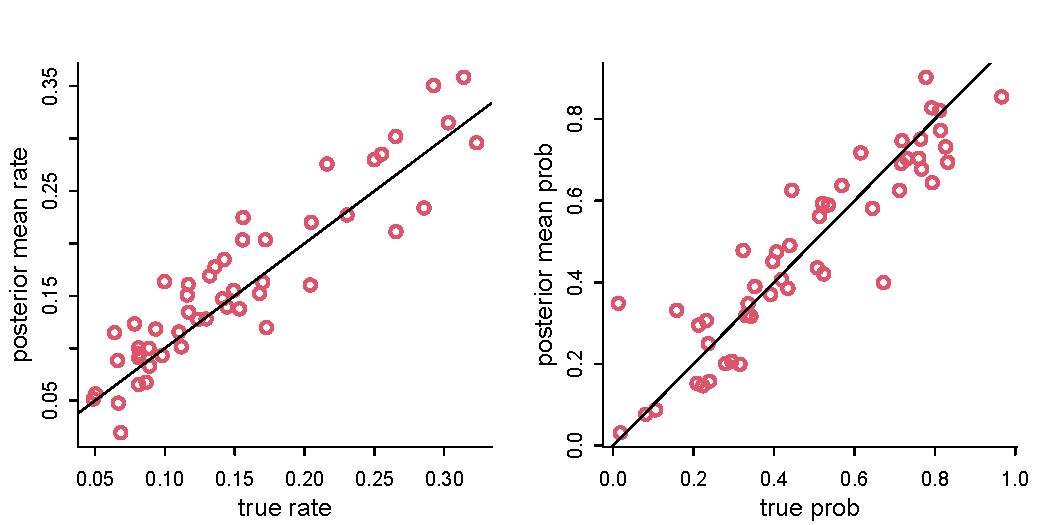
\includegraphics[scale=0.6]{fig_lambda_p.pdf}
\end{center}
The left compares the true $\lambda$ values (horizontal) to the posterior means. The diagonal line shows identity. The right compares the true $p$ parameters (horizontal) to the posterior means. 
This is only one example, but the model unsurprisingly has no trouble estimating Poisson rates and the base rates of each vocalization, except in cases in which a vocalization is never performed in a particular sample.

Now we can ask how the individual repertoires are captured.
\begin{center}
	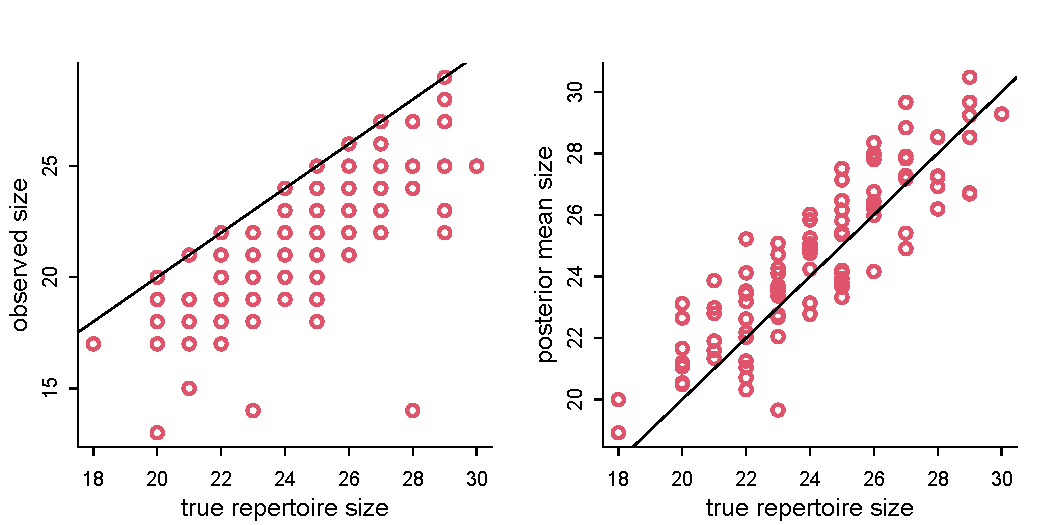
\includegraphics[scale=0.6]{fig_repertoires.pdf}
\end{center}
The left compares the true repertoire size of each individual (horizontal) to the raw observed (vertical). Note the undercounting. The right compares the same true repertoires (horizontal) to the posterior mean sizes. These are still uncertain, but less biased.

%%%%%%%%%%%%%%%%%%%%%%%
\clearpage
\bibliographystyle{apalike} 
\bibliography{references}

\end{document}








